\documentclass[conference]{IEEEtran}
\IEEEoverridecommandlockouts
% The preceding line is only needed to identify funding in the first footnote. If that is unneeded, please comment it out.
\usepackage{cite}
\usepackage{amsmath,amssymb,amsfonts}
\usepackage{algorithmic}
\usepackage{graphicx}
\usepackage{textcomp}
\usepackage{xcolor}
\usepackage{footnote}
\usepackage{multicol}
\usepackage{float}
\usepackage{minted}
\usepackage{todonotes}
\usepackage{url}[hyphens]
\usepackage[acronym, nonumberlist]{glossaries}

\def\BibTeX{{\rm B\kern-.05em{\sc i\kern-.025em b}\kern-.08em
    T\kern-.1667em\lower.7ex\hbox{E}\kern-.125emX}}
\begin{document}

\title{Preliminary evaluation of federated SLURM}

\author{\IEEEauthorblockN{Kees de Jong, Maxim Masterov}
\IEEEauthorblockA{\textit{SURFsara} \\
Amsterdam, The Netherlands \\
kees.dejong@surfsara.nl, maxim.masterov@surfsara.nl}}

\maketitle

\begin{abstract}
\gls{cca} has as a goal to consolidate functionality on a common hardware infrastructure. The hypothesis is that this will create a more cost-effective system, easier management and more flexible access to \gls{hpc} and high performance storage resources. In practice this concept is planned for the integration of Cartesius \cite{cartesius-userinfo} and Lisa \cite{lisa-userinfo} hardware. This research investigated the advantages and disadvantages of a federated \gls{slurm} as a first step of a more unified integration of Cartesius and Lisa.
\end{abstract}

\begin{IEEEkeywords}
Federated SLURM, HPC, unified computing
\end{IEEEkeywords}


\section{Introduction}
\subsection{Background}
\label{sec-background}
\gls{slurm} provides the means to allocate exclusive and/or non-exclusive access to typically \gls{hpc} compute resources for a duration of time \cite{wiki-slurm}. Therefore, \gls{slurm} provides a scheduling framework for starting, executing, and monitoring compute jobs. These are typically parallel \gls{mpi} jobs on a set of scheduled compute nodes. \gls{slurm} also provides the intelligence to manage queues and thus congestion of the compute resources.

Support for creating a federation of clusters was included with the release of \gls{slurm} 17.11. This feature enables users to schedule jobs on a range of clusters with a unified and unique job ID among all clusters \cite{slurm-federated-guide}. Each cluster then independently attempts to schedule the job according to its own scheduling policies. Furthermore, the cluster where the job was submitted to (origin cluster) coordinates with the other clusters in the federation to schedule the job. This is done by submitting copies of the job (sibling jobs) to each eligible cluster.

% What is the general need to have a federated cluster? A PRACE/DEISA federated load leveler project \cite{radecki2014reservations} was not successful due to a lack of need for such a solution [TODO: Citation needed].



\subsection{Experimental setup}
SURFsara intends to integrate the Cartesius and Lisa systems on e.g. the job scheduling level. Federated \gls{slurm} could assist in this ambition. In order to experiment with federated \gls{slurm}, an experimental setup was used (table \ref{tab-experimental-setup}). It is assumed that a true \gls{slurm} federation will not share a uniform setup. Thus, our experimental setup reflects this by using different versions of \gls{slurm} and Linux distributions.

\begin{table}[H]
\begin{center}
\caption{Experimental setup}
\label{tab-experimental-setup}
\begin{tabular}{llll}
\textbf{Cluster name} & \textbf{Linux distribution} & \textbf{SLURM} & \textbf{MariaDB} \\
fedora                & Fedora 31                   & 19.05.4        & 10.3.20          \\
debian                & Debian 10                   & 18.08.5        & 10.3.18          \\
ubuntu                & Ubuntu 18.04.3 LTS          & 17.11.2        & 10.1.29         
\end{tabular}
\end{center}
\end{table}


\subsection{Known limitations}
\label{sec-limitations}
SchedMD (current maintainer of \gls{slurm}) highlighted the following known limitations of a federated cluster \cite{slurm-federated-guide, slurm-federated-cluster-support}.

\begin{itemize}
    \item A federated job that fails due to resources (partition, node counts, etc.) on the local cluster will be rejected and will not be submitted to other sibling clusters even if it could run on them.
    \item Job arrays only run on the cluster that they were submitted to.
    \item Job dependencies are not supported across clusters.
    \item Job modification must succeed on the origin cluster for the changes to be pushed to the sibling jobs on remote clusters.
    \item Modifications to anything other than jobs are disabled in \mintinline{bash}{sview}.
    \item \mintinline{bash}{sview} grid is disabled in a federated view.
    \item Limited size of federation (64 clusters).
    \item JodIDs are stored in 26 bits, not in 32, as in non-federated \gls{slurm}.
    \item A cluster can be a part of only one federation at a time.
    \item Jobs cannot span multiple clusters.
    \item A \gls{slurm} federation is not intended as a high-throughput environment (\textgreater 50,000 jobs a day). However, this can be mediated by using \mintinline{bash}{--cluster-constraint} or the \mintinline{bash}{-M} submission options to limit the amount of clusters the sibling jobs can be submitted to or directing load to.
    \item Job IDs on each cluster are independent (two jobs can have same ID).
    \item No cross-cluster job dependencies.
    \item No job migration between clusters.
    \item No unified view of system state, each cluster largely independent.
    \item \mintinline{bash}{sacctmgr mod cluster} can be used to set a weight on a cluster level, used to prioritize clusters that can start job the soonest.
    \item \mintinline{bash}{sacctmgr mod cluster} can also be used to set features on a cluster level, which can be requested by job.
    \item \mintinline{bash}{sbatch}, \mintinline{bash}{salloc} and \mintinline{bash}{srun} have federation support to submit jobs.
\end{itemize}


\subsection{Research question}
This section briefly discusses the research questions based on the use case and experimental setup (section \ref{sec-background}), and the known limitations (section \ref{sec-limitations}). The term federated \gls{slurm} implies central control over independent clusters. The main research question therefore is; how federated can federated \gls{slurm} actually be and what are the advantages and disadvantages? Furthermore, how applicable is federated \gls{slurm} for the Cartesius and Lisa systems?


\section{Results}
\subsection{Cluster setup}
\label{sec-cluster-setup}
When using \gls{slurm}, a central database may be used to archive job accounting. The daemon used for this is called \mintinline{bash}{slurmdbd}. The \gls{slurm} controller (\mintinline{bash}{slurmctld}) is responsible for monitoring all the \gls{slurm} daemons and resources, accepts work (jobs), and allocates resources to those jobs \cite{slurm-slurmctld}. The \mintinline{bash}{slurmctld} communicates this information to the \mintinline{bash}{slurmdbd} to be archived to a supported database, i.e. MariaDB \cite{mariadb}.
The \gls{slurm} release numbers can be distinguished in two parts, the major release number and the maintenance level. Taking the \gls{slurm} 17.11.2 release number as an example, the first two numbers represent the major release number, while the last of the three represent the maintenance level. The \mintinline{bash}{slurmdbd} must be at the same or higher major release number as the \mintinline{bash}{slurmctld} daemon \cite{slurm-upgrade-guide}. Therefore, the only valid candidate to run the \mintinline{bash}{slurmdbd} in our experimental setup (table \ref{tab-experimental-setup}) is the \mintinline{bash}{fedora} cluster, due to having the highest major \gls{slurm} release number.

Furthermore, \gls{slurm} permits upgrades to a new major release from the past two major releases without the loss of jobs, or other state information. Thus, as also explicitly noted in the official documentation \cite{slurm-upgrade-guide}, the \gls{slurm} versions listed in table \ref{tab-experimental-setup} are compatible. If an older major release ought to be used, then state information and RPCs would not be recognized and discarded, resulting in loss of all running and pending jobs. Therefore, the \mintinline{bash}{slurmdbd} version number can only go up, and in our case a \gls{slurm} version \textless 17.11 would not be compatible (even if those major releases would support federated \gls{slurm}).

If a \gls{slurm} cluster with the highest major release of the \mintinline{bash}{slurmdbd} decides to leave the federation, another cluster has to step in to replace it with a \mintinline{bash}{slurmdbd} major release version that is equal or higher. Otherwise database scheme compatibility problems would arise, a \gls{slurm} downgrade path is not supported. Therefore, the best forward-compatibility is ensured by having the \gls{slurm} daemons in all clusters (regardless of which Linux distribution is used), run the same major version release number. However, we experimented with the versions listed in table \ref{tab-experimental-setup} since the documentation states that these \gls{slurm} versions are compatible.

Across a (federated) \gls{slurm} cluster a uniform user (UID) and group (GID) name space must be assured. This requirement is twofold; to ensure storage permission compatibility throughout the distributed cluster (and network attached file systems), and to ensure that the \mintinline{bash}{SlurmUser} option in \mintinline{bash}{slurm.conf} is mapped to the same numerical UID/GID. Furthermore, accounting is maintained by user name (not UID), however, this also requires uniform user administration across the federated \gls{slurm} cluster \cite{slurm-accounting}. Therefore, all federated \gls{slurm} clusters must use a uniform user administration, e.g. LDAP.

In order to authenticate the UID and GID of another local or remote process (RPC), an authentication mechanism is used called \mintinline{bash}{munge} \cite{github-munge}. The symmetric key used for authentication must be distributed throughout the federated \gls{slurm} cluster. However, it is possible to run multiple \mintinline{bash}{munge} keys by running multiple daemon instances pointing to different keys. Another authentication requirement is time (to prevent replay attacks), thus clocks need to be synchronized throughout the federated \gls{slurm} cluster, this is usually done by NTP.


\subsection{Experimentation}
As discussed in section \ref{sec-cluster-setup}, RPC and state information should be compatible between the \gls{slurm} versions listed in table \ref{tab-experimental-setup}, where the \mintinline{bash}{fedora} cluster acts as the main cluster in the \gls{slurm} federation. However, several errors were observed when the \gls{slurm} federation was created. Before setting up the federated \gls{slurm} cluster, all cluster local jobs completed without issues. However, several errors were introduced after creating the \gls{slurm} federation.

On the \mintinline{bash}{debian} cluster we ran the command \mintinline{bash}{sinfo --federation}, which triggered the \mintinline{bash}{Zero Bytes were transmitted or received} error before showing the expected federated \gls{slurm} cluster overview. However, the output of the command was incorrect. According to the output, the \mintinline{bash}{fedora} and \mintinline{bash}{debian} clusters were running on the same node, while the \mintinline{bash}{ubuntu} cluster was missing from the overview. Similar errors, but with different combinations were observed on other nodes in the federated \gls{slurm} cluster. All \mintinline{bash}{munge} keys were verified with SHA256 and all clocks were syncronized with NTP. The \mintinline{bash}{slurmdbd} log on the main cluster registered the error \mintinline{bash}{federation siblings not synced yet}. Network connections, \gls{slurm} daemon and database permissions were verified. However, the errors persisted.

Therefore, as recommended by ourselves in section \ref{sec-cluster-setup}, we setup a federated \gls{slurm} cluster with the same major release versions.








\section{Discussion}
% discuss what was done
% discuss the findings
% discuss infrastructure specific variable such as; mounted file systems, paths to certain software or data

% \begin{figure}[H]
% \centering
% 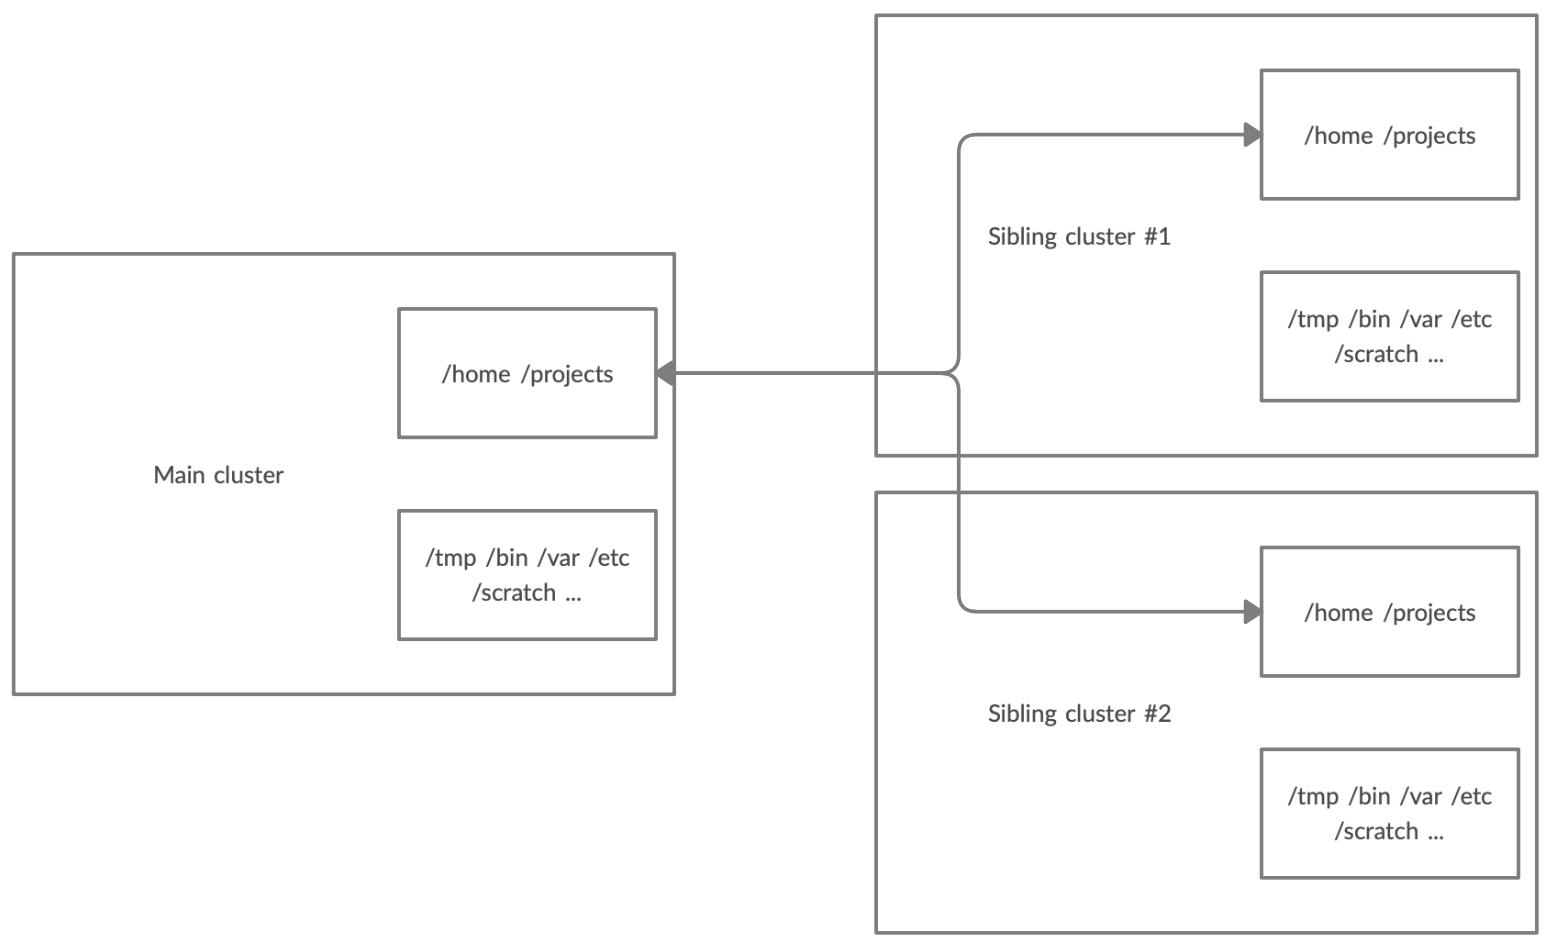
\includegraphics[width=\columnwidth]{images/file_system.png}
% \caption{Uniform cluster setup.}
% \label{fig-cluster-setup}
% \end{figure}



\section{Conclusion}
% evaluate the findings discussed in discussion with the known limitations
% conclude the pros and cons
% briefly discuss the prace unicore project and the leassons we can learn from that based on the findings of this rapport


\section{Future work}
% list the stuff that we intended to do, but didn't conclude due to time restrictions
% compare functionality and success of unicore





\newacronym{slurm}{SLURM}{Simple Linux Utility for Resource Management}
\newacronym{cca}{CCA}{Central Converged Architecture}
\newacronym{hpc}{HPC}{High Performance Computing}
\newacronym{mpi}{MPI}{Message Passing Interface}


\bibliographystyle{./bibliography/IEEEtran}
\bibliography{./bibliography/IEEEabrv,./bibliography/IEEEexample}

\end{document}